\section{Theory}
\label{sec:Theorie}

\subsection{Diode Laser}

A Diode Laser is used in the Experiment.
In Princepal the Laser consists of three main parts.
\begin{itemize}
    \item An active Medium
    \item A pump
    \item A Resonator
\end{itemize}

The \textbf{active Medium} consists of a \textbf{p-type} and an \textbf{n-type} Semiconductor.
A semiconductor has a conductivity that falls between that of an insulator and a conductor.
This property can be explained by the Band model. 
As a result of the cristall structure of condensed matter all of the atoms in the cristall are very close together which would mean that their electrons would share the same quantum state.
The pauli exclusion principal forbids this so the energy state of the electrons slightly change.
The result is the so called electronic band structure.
This means that a lot of energy levels are almost the same, these energy level can be discribe as one band.
After one band there is a band gap in which no possible energy levels lie after the gap next band starts.
\\
The highest band that's still occupied by electrons at the Fermi level, so at absolute zero temperature, is called the valence band.
The conduction band is the band that follows the valence band.
In metals the properties of those two bands are combined, because the Fermi energy lies inside a band as shown in graphic \ref{fig:band_structure}.

\begin{figure}
    \centering
    \caption{The band structure of diffrent types of condensed matter, the shades follow the Fermi-Dirac distrubution of the elctrons in the given material. The graphic is taken from source \cite{wikipedia_valence_conduction_band}}
    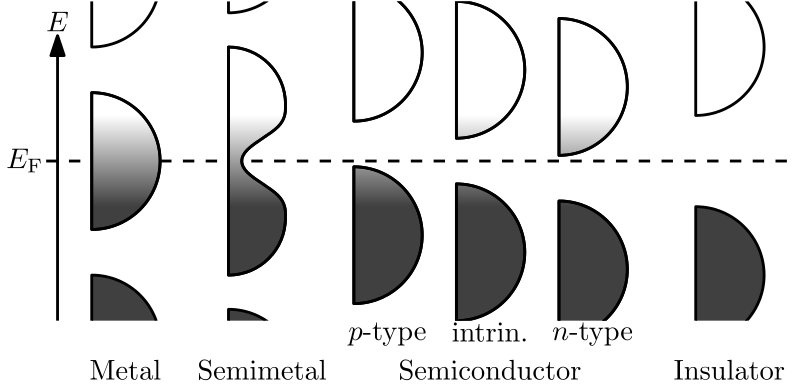
\includegraphics[width=0.75\textwidth]{content/data/Band_structure_diffrent_materials}
    \label{fig:band_structure}
\end{figure}

In semiconductors those bands are distinc from another so the conduction band lies above the Fermi level and the valence band beneath.
This means at absolute zero the semiconductor does not conduct.
With rising temperature more electrons move from the valence band into the conduction band so the semiconductor gains the property to conduct.
This property alone is not usefull on it's one for building a laser.
To modify the conductivity and properties of the semiconductor, impurities get introduced into into thier crystal lattice.
Depeding on the material used the result is called a p-type or n-type semiconductor.
this process is called doping.
\\\\
\FloatBarrier
For a \textbf{p-type} semiconductor a impurity is used that has less valence electrons than the material that builds the semiconductor cristall.
This way a missing charge forms that can freely move thorugh the cristall and behaves like a positive charge, that is why p-type semiconductor are also called Acceptors.
A picture visualizing the p-type doping is shown in graphic \ref{fig:p-type_doping}.
As seen in the picture the Boron has one less valence electron so it can not form a covalent bond with the silicon on it's right.
This results in a void wich is a missing charge that can move thorugh the cristall.

\begin{figure}
    \caption{Through diffrent doping materials it's possible to achieve p-type and n-type semiconductors, as shown in the pictures.}
    \begin{subfigure}{0.48\textwidth}
        \centering
        \caption{A 2 dimensional scheme, of a p-type semiconductor made of silicon, doped with Boron. The picture is taken from source \cite{p-type_doping}.}
        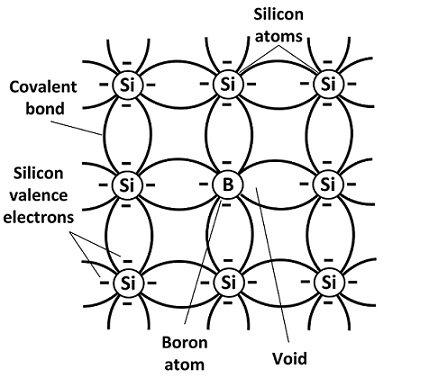
\includegraphics[height=5cm]{content/data/p-type-semiconductor-doping}
    \label{fig:p-type_doping}
    \end{subfigure}
    \hfill
    \begin{subfigure}{0.48\textwidth}
        \centering
        \caption{A 2 dimensional scheme, of a n-type semiconductor made of silicon, doped with antimony. The picture is taken from source \cite{p-type_doping}.}
        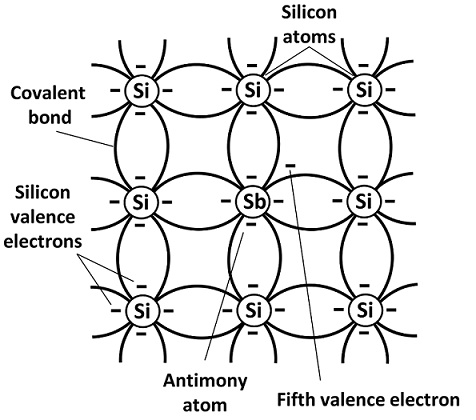
\includegraphics[height=5cm]{content/data/N-Type-Semiconductor-Doping}
        \label{fig:n-type_doping}
    \end{subfigure}
    \label{fig:p-n-type_doping}
\end{figure}


Doping is also possible with an impurity that hase an valence electron more than the cristalls material.
In that case the electron that can not form a covalent bond is able to move freely thorugh the cristall.
The result is a free negativ charge. In this case the semiconductor is called an \textbf{n-type} semiconductor, or Donor.
The picture \ref{fig:n-type_doping} shows an n-type semiconductor made of silicon which is doped with antimony.
The result is a fith valence electron that can not form a valence bond and in return is able to move trough the cristall.
\\\\
\FloatBarrier
If now a p-type and an n-tpye semiconductor are brought together the free electrons from the n-type semiconductor tend to move into the holes of the p-type semiconductor.
This results in emission of photons, because the energy of the n-type electrons is higher than the energy states in which they drop in the p-type semiconductor.
This process is used as active medium in the Diode laser.
\\\\
But the active medium alone is not of much use, because the flow of electrons from n-type to p-type stops after a short while.
This is because an equilibrium forms.
To keep the elctrons moving they have to be brought back into the n-type semiconductor.
So they have to be pumped up into the higher energy state they had before the moved into to the p-type semiconductor.
The \textbf{pump} is made up by applying an electric field to both semiconductor layers.
With the electric field the electrons move back into the n-type semiconductor to start the cycle over again.
\\\\
With the pump and the active medium alone the laser would already emitt light but that light is not coherent, so the basic property of laser light is still missing.
To make the laser just emitt coherent light a resonator is used.
\\\\
A \textbf{resonator} consists of two reflectiv layers that engulf the active medium.
The distence between those mirrors is choosen to be $n \lambda/2 = L$ with $n$ as natural number, $\lambda$ the wavelength of the laser light and $L$ the distance between the mirrors.
This way, whenever light gets emitted by the active medium its trapped between the reflectiv layers and forms a standing wave.
The photons than bounce back and forth in the resonator and provide a feedback for the active medium.
Which results in the emission of more photons with the same characteristics as the initial photons.
In the Diode laser the resonator consists of a cavity that is made up by two cleaved facets at the ends of the diode chip.
Depending on the coating of these the reflectivy increases or decreases.
\\\\
With all these componentes the Diodelaser emitts laser light with a wavelength near $\lambda = \SI{785}{\nano\meter}$, with an output power of about $P_\text{laser} = \SI{70}{\milli\W}$.

\subsection{Diffraction Grating}
Bare Diodelaser emitt light with a large bandwith $\Delta f_\text{laser} = \SI{50}{\mega\Hz}$, which is large compared to the linewidths of atomic transitions $\Delta f_\text{atomic} = \SI{5}{\mega\Hz}$.
They are also very sesitive to optical feedback, so it's not desirable to reflect any light back into the internal Laser cavity.
To solve this problem a Diffraction Grating is installed infront of the laser, as shown in graphic \ref{fig:grating}.

\begin{figure}
    \centering
    \caption{A grating is installed infront of the laser to prevent outside feedback aswell as shortening the bandwidth of the laserlight. The graphic is taken from source \cite[5]{anleitung_laser}}
    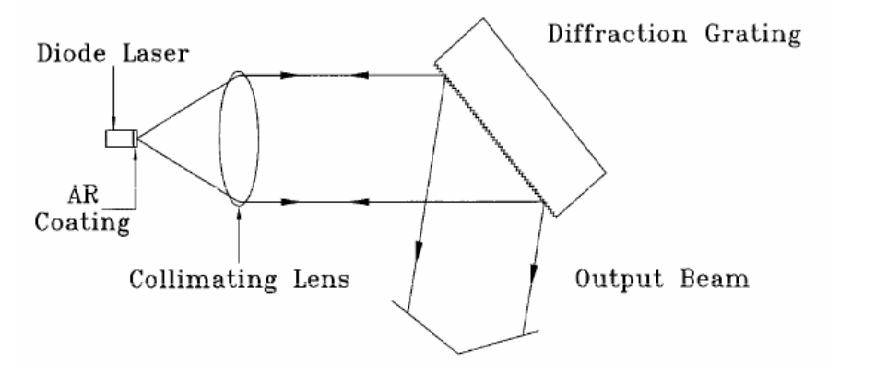
\includegraphics[width=0.75\textwidth]{content/data/grating}
    \label{fig:grating}
\end{figure}

About $85\%$ of the light that hits the garting gets reflected, this light has grating order $m=0$.
The other $15\%$ are reflected back into the laser to form an extrenal cavity.
The light that's reflected back into the laser is of grating order $m=1$.
Light that tarvels back into the laser stabilizies the frequenzy of the laser and narrows the linewidth to less than $\Delta f_\text{laser} = \SI{1}{\mega\Hz}$.


\subsection{Laser tuning}
Because the laser always tends to lase in the frequenzy with the greatest net gain we want to find that frequenzy.
This frequenzy depends on four factors 

\begin{itemize}
    \item The medium
    \item The internal cavity
    \item The Grating Feedback
    \item The External cavity.
\end{itemize}

\begin{figure}
    \centering
    \caption{The net gain of every componentes should peak at the wavelength $\lambda_0$, the net gain of every component is shown in this picture. The picture is taken from source \cite[6]{anleitung_laser}.}
    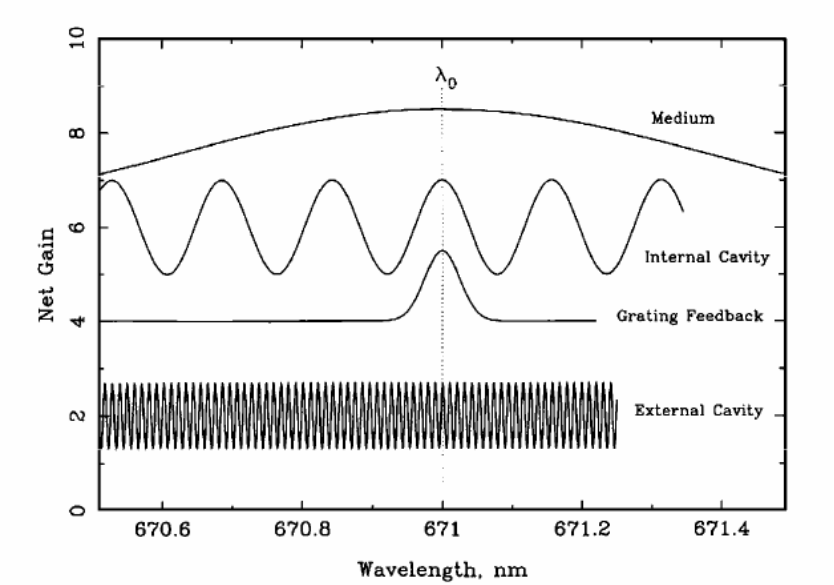
\includegraphics[width=0.75\textwidth]{content/data/netgain}
    \label{fig:netgain}
\end{figure}

\subsubsection{Medium gain}
All these factors have an influence on the net gain and with that on frequenzy of the laser.
A graphic illustrating the diffrent influence is visible in garphic \ref{fig:netgain}.
The medium gain depends on the properties of the semiconductor and also depends on the temperature of the laser.
But because the temperature of the laser will be determined in the Experiment we can assume that the medium lases with a wavelength of about $\SI{785}{\nano\meter}$ as mentioned before.

\subsubsection{Internal cavity gain}
The internal cavity adds an influece onto the frequenzy of the laser.
It's net gain is frequenzy dependent, as shown in figure \ref{fig:netgain}.
The period is defined by the length of the cavity $L$, the index of refraction $n$ and is given by
$\Delta f_\text{int} = \frac{c}{2Ln}$.

\subsubsection{Grating gain}
The grating can be shifted.
That way only the light from a narrow wavelength band will be fed back into the cavity.
The lights wavelength can be found by the bragg condition $\lambda = \frac{2d \sin{\theta}}{n}$ with the atomic spacing $d$, the diffraction order $n$ and the glancing angle $\theta$.
Because the diffraction order $n = 1$ we can write the bragg condition as $\lambda = 2d\sin{\theta}$.
With this the $\Delta f$ is given by $\frac{f}{\Delta f} = N$ with $N$ as the number of grating lines subtended by the laser beam.
In the Experiment $N=5400$ which results into $\Delta f \approx \SI{70}{\giga\Hz}$.

\subsubsection{External cavity gain}
The extrenal cavity is made up by the garting and the back facet of the diode.
Similar to the internal cavity it's net gain also periodicly shifts, with $\Delta f = \frac{c}{2L}$.
\\
But the distance is larger than that of the internal cavity which results to $\Delta f_\text{ext} \approx \SI{10}{\giga\Hz}$.
Because the period is dependent on the distance between the garting and the diode the period also changed when the garting is moved.
\\\\
Forcing the laser into lasing with a single mode is achieved by chnaging the net gain of every component discussed before to the wavelength $\lambda_0$ of the medium.
The optimal case is pictured in graphic \ref{fig:netgain}, as every net gain peaks at $\lambda_0$.

\subsection{Absorption from Rubidium}
Photons have the ability to raise the energy state of electrons in atoms.
After some time the electron falls back to its initial state and emitts light with the frequenzy/wavelength as the photon that started the process.
The electron can also move back into its initial state by falling back into its initial state in multiple steps, realising multiple photons doing so, just the sum of energy must be the same.
The material that absorbs light in this Experiment is Rubidium more specific $\ce{^{85}Rb}$ and $\ce{^{87}Rb}$.
There Absorption spectrum lies with in the wavelength of the laser used in the experminet.
